\vspace*{-1mm}

\section{Emittance}

\textbf{Defintion 1}: The statistical emittance is expressed in terms of the beam distribution: % Wolski Eq. (4.101)

\begin{equation}\label{eq:statistical_definition_emit}
    \epsilon_x^{\mathrm{geom}} = \sqrt{\langle x^2 \rangle - \langle px^2 \rangle - \langle x px \rangle^2}.
\end{equation}
This is the geometric emittance. 
\begin{equation}\label{eq:emit_geom_norm_relation}
    \epsilon_x = \epsilon_x^{\mathrm{geom}} \betarel \gammarel.
\end{equation}


\textbf{Defintion 2}:
For a gaussian beam distribution the normalised beam emittance it applies:
\begin{equation}\label{eq:emit_from_beam_size}
    \epsilon_{x} = \frac{\sigma_x(s)^2 - \delta^2 D_x^2(s)}{\beta_x(s)} \betarel \gammarel
\end{equation}

where $\sigma_x(s)$ is the beam size, $\beta_x(s)$ is the beta function, $D_x(s)$ is the dispersion fat a specific location s along the accelerator, $\delta=\Delta p/p0$ is the momentum spread and $\betarel, \gammarel$ the relativistic parameters. Similar expression is valid for the vertical plane, with the difference that there is no dispersion.

\section{Transfer maps}
Need to mention them briefly as you refer to them at the PyHEADTAIL section.

\section{Action angle variables}
The action for the x-plane is:

\begin{equation}\label{eq:action}
    \Jx = \frac{1}{2}(x_n^2 +xp^2_n) 
\end{equation}
where 
\begin{equation}\label{normalised_y}
    x_n = \frac{x}{\sqrt{\beta_x}}, \ \ xp_n = \frac{\alpha_x x}{\sqrt{\beta_x}} + \sqrt{\beta_x}xp
\end{equation}
the normalised coordinates and $\alpha_y, \beta_y$ the twiss parameters. 
The same applies for the y-plane. 

s
The statistical geometric emittance equals the average of the actions distribution:
\begin{equation}\label{eq:geom_emit_actions}
    \emitxgeom = \langle \Jx \rangle
\end{equation}
%\begin{equation}\label{eq:geom_emit_actions}
%    \epsilon_x^{\mathrm{geom}} = \langle \Jx \rangle
%\end{equation}
The distribution of actions is an exponential distribution (further explanation needed?). Therefore, its mean equals its standard deviation. (this property is used in the appendix for the computation of the rms tune spread.)

From Eq.~\eqref{eq:action} we write:
\begin{equation}\label{eq:Jy_exp_distr}
    e^{-J/\epsilon} = e^{(-x^2/2\epsilon - px^2/2\epsilon)}
\end{equation}
From this equation it can be seen that the actions follow an exponential distribution. 

\section{Wakefields and impedances}\label{sec:wakefields_theory}

he terms dipolar and quadrupolar have been chosen as the dipolar wake function acts on the test proton like a dipole magnet (the kick is the same whatever its transverse location), whereas the quadrupolar term acts like a quadrupole magnet (the kick increases linearly with the transverse offset of the test particle). Benoits thesis p.44


\section{Tracking simulation codes}\label{sec:simualtion_codes}
In this section the two tracking simulation codes used in this thesis to study the noise-induced emittance growth are presented. Both codes are macroparticle tracking libraries that simulate the particle motion in the six-dimensional (6D) phase space $(x, p_x, y, p_y, z, \delta)$. The first code performs tracking between interaction points around a circular accelerator with the use of trasnfer matrices while the second one uses the detailed optics model of the machine.

\subsection{PyHEADTAIL}\label{subsec:pyheadtail}

PyHEADTAIL~\cite{pyheadtail_repository, pyheadtail_manual_adrian} is an open-source 6D macroparticle tracking code which was originally designed to study collective effects in circular machines and to be easily extrensible with custom elements.
% https://indico.cern.ch/event/930271/contributions/3910265/attachments/2066139/3467770/30June2020_Simulations_emit_growthCC_RFnoise.pdf  
The following paragraphs provide a brief overview of the basic modules of PyHEADTAIL and of the procedure to build and run the simulation according to the detailed description in Refs.~\cite{pyheadtail_schenk, Schenk:2665819}.

To begin, a particle bunch is represented by a collection of macroparticles, each of which represents a clustered collection of physical particles. Each macroparticle is described by four transverse $(x, p_x, y, p_y)$ and two longitudinal coordinates $(z, \delta)$, a mass and an electric charge. For the studies presented in this thesis  $10^{5}$ macroparticles are sufficient for an accurate represantation of the bunch, unless it is stated otherwise.

The accelerator ring is represented by an one-turn map splitted into a number of segments of equal length, after each of which there is an interaction point. At the interaction points the macroparticles experience kicks from various accelerator components (feedback system, multipoles etc) or from collective effects such as the wakefields. In the transverse plane, the macroparticles are transported from one interaction point to another by linear transfer matrices which take into account the optics parameters at the beginning and the end of the respective segment. The matrices can include detuning feutures from chromaticity and amplitude detuning as a change of phase advance of each macroparticle. Last, the tracking in logitudinal plane is performed with linear or non-linear synchrotron motion. In this thesis, a linear longitudinal one-turn map is used represented by a Courant-Snyder trasnfer matrix and using only the linear first order slippage factor. %Last sentence from (LinearMap): https://github.com/PyCOMPLETE/PyHEADTAIL/blob/master/PyHEADTAIL/trackers/longitudinal_tracking.py
During the tracking the bunch data are available at the end of the last segment every turn. Figure~\ref{fig:pyheadtail_accelerator_model} shows a graphic representation of the accelerator model and the tracking procedure.
% Graph is created app.diagrams.net and is saved in goodle dirve.

\begin{figure}[!h]
    \centering         
    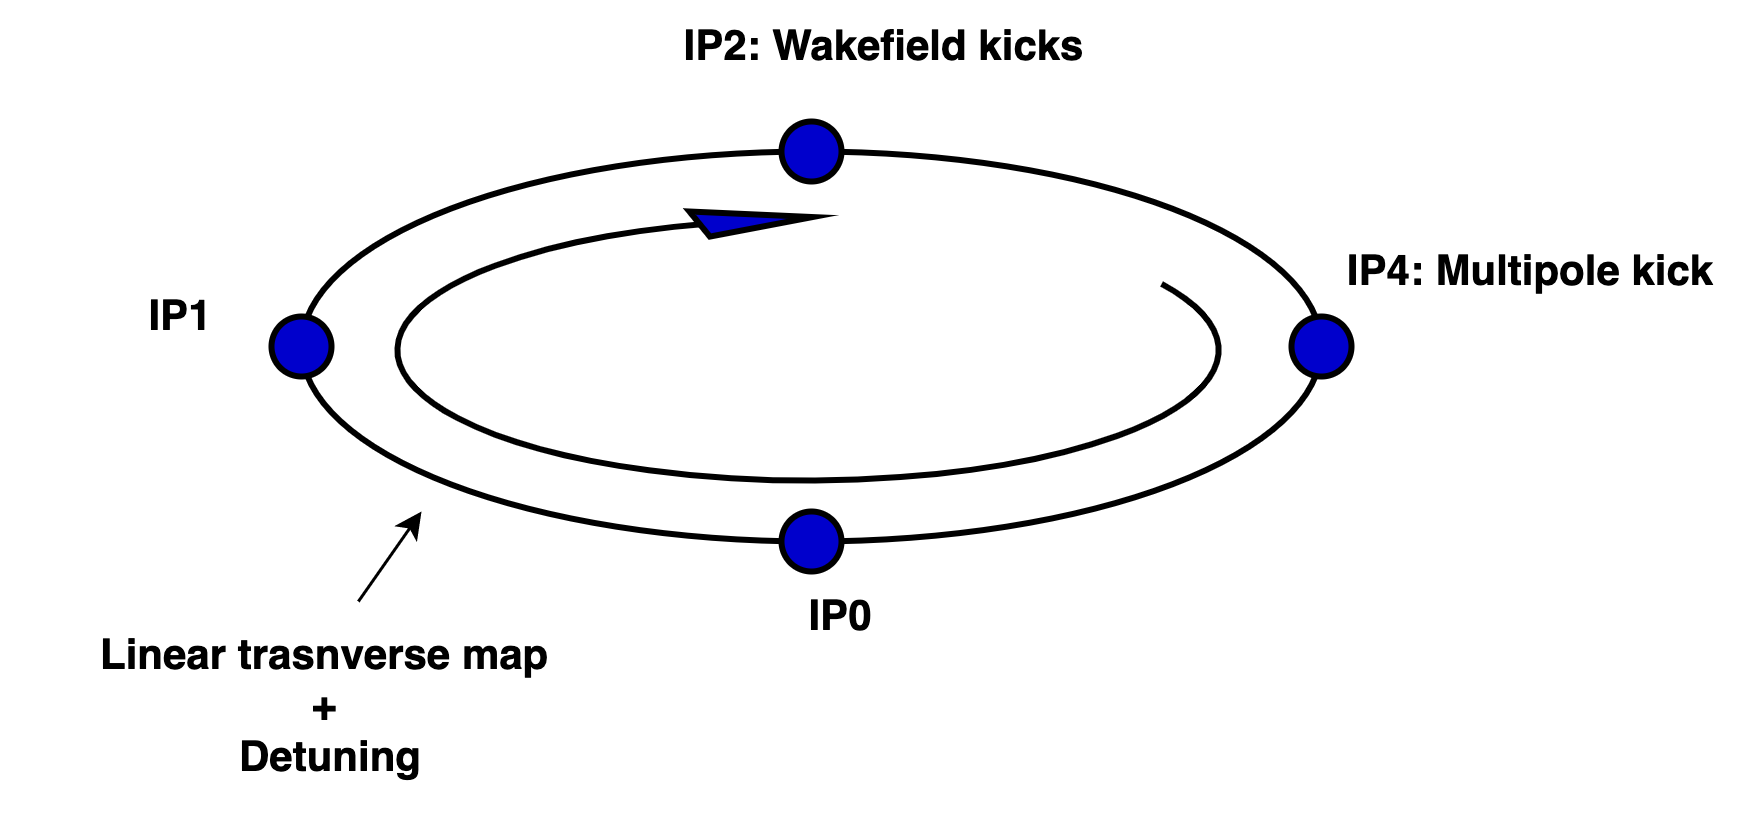
\includegraphics[width=0.6\textwidth]{images/Ch2/accelerator_model_graph_pyheadtail.png}
        \caption{Graphic represantation of the accelerator model and tracking procedure in PyHEADTAIL (inspered by the graphs in Refs.~\cite{pyheadtail_schenk, inproceedings_ibs_pyheadtail}). In this example the ring is splitted in four segments. The blue points correspond to the interaction points while the curved arrow shows the direction of the beam during the tracking.}
        \label{fig:pyheadtail_accelerator_model}
 \end{figure}


\subsection{Sixtracklib}\label{subsec:sixtracklib}
%Introduction to sixtrackib: https://indico.cern.ch/event/833895/contributions/3577803/attachments/1927226/3190636/intro_sixtracklib.pdf
% https://inspirehep.net/files/6273430c727ace3796a92d069f651ade